\documentclass[a4paper,12pt]{book}
\usepackage[utf8]{inputenc}
\usepackage[english]{babel}
\usepackage{graphicx}
\usepackage{algorithm2e}
\usepackage{tikz}
\usepackage[nottoc]{tocbibind}
\usepackage[backend=bibtex,style=alphabetic,citestyle=authoryear]{biblatex}
\usepackage[linktocpage=true]{hyperref}
\usepackage{appendix}
\usepackage{amsmath}
\usepackage{bm}
\addbibresource{./Bibliography/DataStructuresAndAlgorithms.bib}
% !TeX spellcheck = en_US

\begin{document}

\author{Christian Popescu}
\title{Notes on Data Structures and Algorithms}
\date{November 2019}

\frontmatter
\maketitle
\tableofcontents
\setcounter{secnumdepth}{5}
%\setcounter{tocdepth}{5}

\mainmatter
% !TeX spellcheck = en_US
\part{Data Structures}

% !TeX spellcheck = en_US
\chapter{The First Chapter}
\section{Priority Queues}
% !TeX spellcheck = en_US
\chapter{Sorting}
\section{Merge sort}

It is an example of \textbf{divide and conquer} strategy.

\section{Quick sort}
The quicksort algorithm has a worst-case running time of $\Theta(n^{2})$ on an input array of n numbers.

Applies \textbf{divide and conquer} strategy.

\section{Heap sort}
% !TeX spellcheck = en_US

\chapter{Trees}

\section {General Trees}

A \textbf{tree} is an abstract data type that organize  elements hierarchically.

A tree is \textbf{ordered} if there is a meaningful order among the children of each node.

\section{Binary Tree}

A \textbf{binary tree} is an ordered tree in which any node could have at most 2 children.

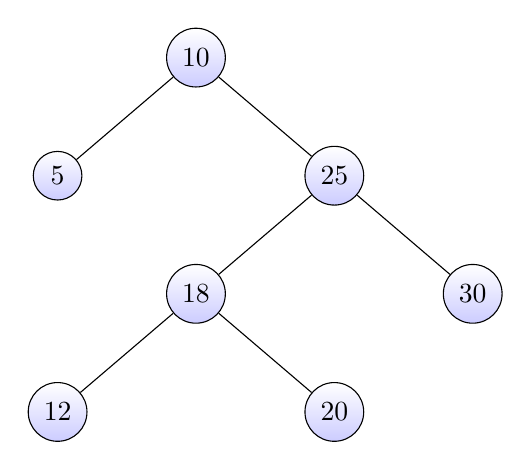
\begin{tikzpicture}[sibling distance=10em,
every node/.style = {shape=circle,
	draw, align=center,
	top color=white, bottom color=blue!20}]]
\node {10}
child { node {5} }
child { node {25}
	child { node {18}
		child { node {12} }
		child { node {20} } }
	child { node {30} } };
\end{tikzpicture}

\subsection{Implementation}
\lstset { %
	language=C++,
	backgroundcolor=\color{black!5}, % set backgroundcolor
	basicstyle=\footnotesize,% basic font setting
	tabsize=4,
}

\color{blue}
\begin{lstlisting}

class BinaryNode {
	public:
	BinaryNode* left;
	BinaryNode* right;
	BinaryNode* parent;
	int key;
};
\end{lstlisting}
\color{black}
\section{Binary Search Tree}

As the number of children of one node is at most 2 we can keep direct links to them.

For some algorithms the navigation up in the tree is required so we can keep a link to the parent node.

\section{Tries (Prefix trees)}

A \textbf{trie} is a variant of a n-ary tree in which characters are stored at each node.  

\cite{latexcompanion}


% !TeX spellcheck = en_US
\chapter{The Second Chapter}
% !TeX spellcheck = en_US
\chapter{Graph algorithms}
\section{Breadth-first search (BFS)}
The algorithm use a \textbf{Queue} to manage the gray vertices. 
% !TeX spellcheck = en_US
\part{Algorithm Techniques}

% !TeX spellcheck = en_US
\chapter{Backtracking}
\section{Problem's specification}

Pattern:

For a given problem we search all the sequences  $\bm{x_{1}x_{2} ... x_{n}}$ for which some property holds
 $\bm{P_n(x_{1},x_{2}, ..., x_{n})}$

\bigskip where: $\bm{x_k \in D_k}$ (some given domain of integers )
\\
The backtrack method consists in designing "cutoff"/"bounding" properties $\bm{P_l(x_{1},x_{2}, ..., x_{l})}$ for $\bm{1\leq l < n}$ such that: 

\begin{itemize}
 \item $\bm{P_l(x_{1},x_{2}, ..., x_{l})}$ is true whenever $\bm{P_{l+1}(x_{1},x_{2}, ..., x_{l+1})}$ is true;
 \item $\bm{P_l(x_{1},x_{2}, ..., x_{l})}$ is simple to test, if $\bm{P_{l-1}(x_{1},x_{2}, ..., x_{l-1})}$ holds.
 
\end{itemize}

\section{Algorithm}
\subsection{Recurisive version}
\SetKwProg{Fn}{Function}{}{end}\SetKwFunction{FRecurs}{FnRecursive}%
\SetAlgoLongEnd
\begin{algorithm}
\Fn{Backtracking}
\end{algorithm}


\section{References}

Bactracking from \cite{KnuthArtOfCompProg4-5b}

\backmatter
% bibliography, glossary and index would go here.
\begin{appendices}
	
	\chapter{Supplementary Information}
	
	\section{Tables}
	
	\section{Figures}
	
	\chapter{References}
	
\printbibliography
	
%	\bibliographystyle{abbrv}
	
\end{appendices}
\end{document}